\subsubsection{Jockey Screen Flow}

\begin{figure}[H]
    \centering
    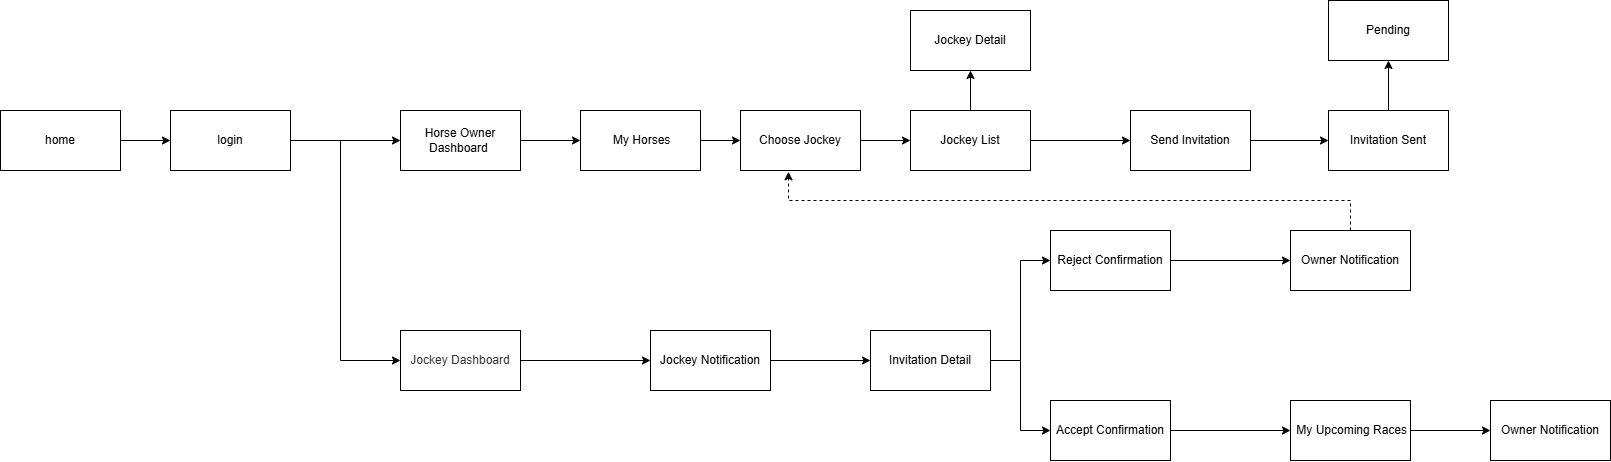
\includegraphics[width=0.9\textwidth]{figures/srs/jockey_Requirements/screenflow_jockey.png}
    \caption{Jockey screen flow}
    \label{fig:jockey_screen_flow}
\end{figure}

\subsubsection{Jockey Screen description}

\TableStart{|p{0.05\textwidth}|p{0.18\textwidth}|p{0.20\textwidth}|p{0.47\textwidth}|}
\textbf{\#} & \textbf{Feature} & \textbf{Screen} & \textbf{Description} \\
\hline
1 & General & Home & Landing page for all users; navigate to Login. \\
\hline
2 & General & Login & Authenticate the jockey and enter the Jockey Dashboard. \\
\hline
3 & Dashboard & Jockey Dashboard & Main hub for jockey with navigation to invitations, upcoming races, results, and profile. \\
\hline
4 & Notifications & Jockey Notification & View pending invitations from owners with horse, owner, tournament, and current status. \\
\hline
5 & Invitation & Invitation Detail & Display invitation details including owner, horse, tournament, schedule, and custom message. \\
\hline
6 & Invitation & Accept Confirmation & Confirm acceptance of the invitation and register the jockey for the selected race. \\
\hline
7 & Invitation & Reject Confirmation & Decline the invitation and send notification back to the owner. \\
\hline
8 & Schedule & My Upcoming Races & Show accepted races with date, time, horse, owner, tournament, and race status. \\
\hline
9 & Notification & Owner Notification & Notify the owner whether the invitation was accepted or rejected. \\
\TableFinish{Jockey screen descriptions}{tab:jockey_screen_screens}
